\section{引言}

机器人完成一条指定轮廓，既需要求出末端位置与关节角的对应关系，也需要计算驱动器应提供的力矩。正运动学回答“给定关节角，末端在哪里”，逆运动学回答“到达目标点需要怎样的关节角”，雅可比矩阵则把这两类位置关系延伸到速度与力的映射。动力学进一步考虑质量、转动惯量和重力，使轨迹规划能够与驱动负载联系起来。对于并联机器人，还必须满足多条支链在同一末端处的闭环约束。因此，仅展示一条能够画出的曲线，尚不足以说明机器人能够平稳、可靠地执行该任务。

本文选择具有实际绘图和教学应用背景的平面五杆机器人，研究其在竖直工件板面上描绘椭圆轮廓的设计问题。实物平台与设计场景的对应关系在第2.1节说明。五杆机构由两条2R串联支链连接同一末端构成，既保留双连杆运动的直观几何关系，又包含闭链机构特有的工作模式、装配模式和并联奇异性，适合在同一案例中贯通课程内容。MIT机器人课程讲义直接以五杆机构说明串联支链组成并联机构的方式；Modern Robotics则提供运动学、静力学和受约束动力学的统一框架\cite{asada2005,lynch2017}。

针对五杆机构，已有研究系统讨论了对称5R机构的运动学、奇异性与工作空间\cite{liu2006}。这些理论提示了一个与实际描绘任务直接相关的问题：目标点虽然位于几何可达域内，机构仍可能接近闭环奇异位形，导致速度、误差和驱动力矩的映射显著恶化。本文不提出新的机构理论，而是围绕这一问题完成可核查的推导和计算：先将左侧支链作为独立2R开链，建立DH运动学、雅可比及拉格朗日动力学；再以独立牛顿—欧拉递推进行交叉核验；随后恢复五杆闭环，推导并联正逆解与两类奇异性，并通过虚功把支链动力学组装为整机模型；最后比较常规描绘轨迹与近奇异轨迹，分析工作空间选择对驱动负载的影响。

\section{系统建模与理论推导}

\subsection{实际机器人背景、任务场景与参数}
\label{sec:system}

实际参照平台为Quanser公司的2 DOF Planar Robot绘图实验机器人，如图\ref{fig:real_robot}所示。制造商介绍与用户手册表明，该设备采用五杆并联机构，两台带减速器的电机驱动基座关节，公共末端安装笔，并由电磁机构完成落笔，以纸上轨迹展示机器人运动效果\cite{barnard2009,quanser2013}。因此，轮廓描绘不仅是抽象的点轨迹，也对应真实设备中的笔尖定位任务。

\begin{figure}[htbp]
\centering
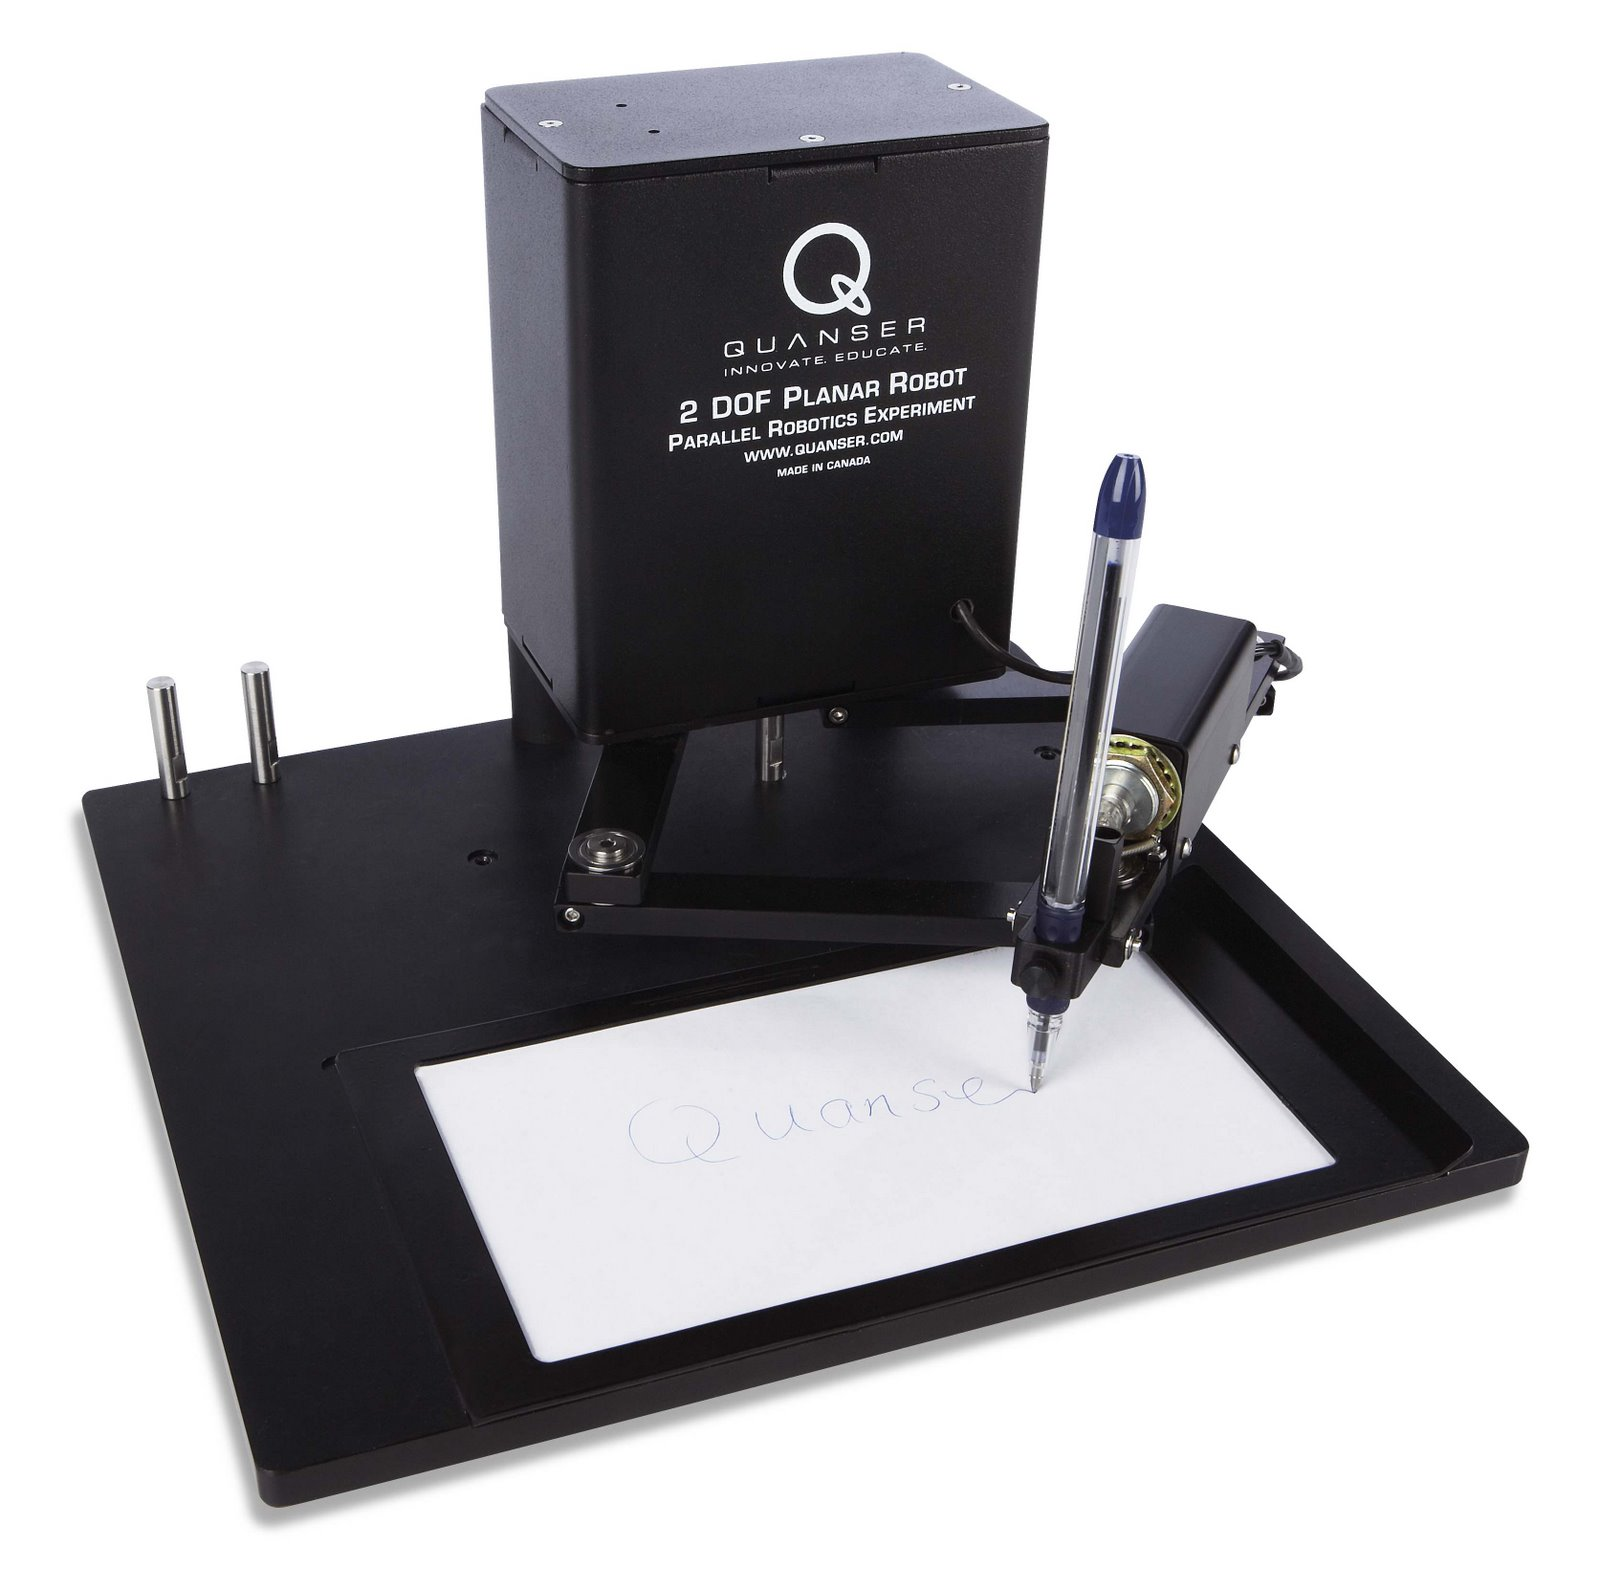
\includegraphics[width=0.66\linewidth]{Quanser_2009_2DOF_Planar_Robot_official_blog.jpg}
\caption{Quanser 2 DOF Planar Robot实物及笔式绘迹配置。来源：制造商官方工程博客，Barnard，2009\cite{barnard2009}；\textcopyright\ Quanser，原图未修改，作为实际机构与应用场景的引用图片。}
\label{fig:real_robot}
\end{figure}

本文保留该平台的五杆拓扑与笔式绘迹需求，进一步设定一个竖直工件板上的椭圆轮廓标记场景：工具在宽$80\units{mm}$、高$50\units{mm}$的轮廓上运动，并在$4\units s$内从静止出发、闭合后回到静止。与桌面绘图相比，竖直安装使杆件和工具的重力直接参与板面内负载，适合分析拉格朗日和牛顿—欧拉方程中的重力项。表\ref{tab:parameters}所列尺寸、质量及安装方向均为本报告的课程设计输入，未将其标作Quanser原机规格，也不将数值仿真表述为原机实测或参数复现。

在工程实施中，完整描绘流程还包括定位板面、抬笔到起点、落笔、沿轮廓运动与抬笔退出。本文研究其中落笔后的二维轮廓段；法向落笔行程作为独立动作，不引入二维模型的自由度。安装方向的影响将在第3节用同一机构从水平到竖直的倾角扫描进行定量说明。


\begin{figure}[htbp]
\centering
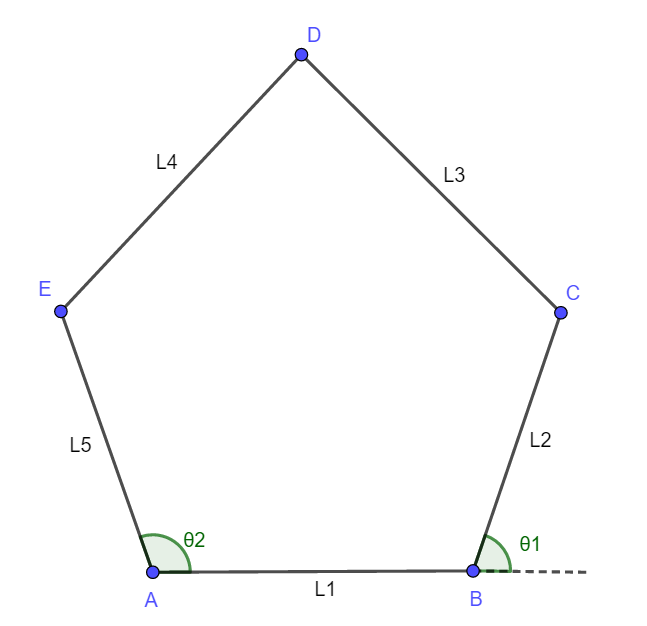
\includegraphics[width=0.57\linewidth]{Five_bar_mechanism_I_Elgamal_2020.png}
\caption{五杆闭链机构的公开示意图。原作者I.Elgamal，2020，原图未修改\cite{elgamal2020}；采用\href{https://creativecommons.org/licenses/by-sa/4.0/}{CC BY-SA 4.0}许可。原图字母与本文建模符号分别定义。}
\label{fig:external}
\end{figure}

本文模型如图\ref{fig:model}所示，固定基座为$A=(-d/2,0)^\T$和$B=(d/2,0)^\T$，肘关节为$C$、$D$，末端公共转动副为$P$。两侧近杆长度均为$l_1$，远杆长度均为$l_2$。世界坐标$x$向右、$y$向上，所有角度逆时针为正。机架$AB$与四根运动杆共五个构件，五个转动副约束平面刚体运动，自由度为
\begin{equation}
F=3(n-1)-2j=3(5-1)-2\times5=2.
\end{equation}
该计数适用于一般非退化位形；奇异位形还须检查约束矩阵的秩。驱动器位于$A$、$B$，两个主动角记为$\vect\theta=(\theta_L,\theta_R)^\T$。左、右支链各用相对关节坐标$\vect q_i=(q_{1i},q_{2i})^\T$表示，其中$q_{1L}=\theta_L$、$q_{1R}=\theta_R$，远杆绝对角为$q_{1i}+q_{2i}$。末端只控制平面位置，不能另外独立指定工具在平面内的姿态。

\figfull{fig01_mechanism.pdf}{本文五杆机器人设计模型。两主动关节位于固定基座，$q_{2L}$为左支链相对角；长度与质量采用表\ref{tab:parameters}中的课程设计值。}{fig:model}

\begin{table}[htbp]
\centering\caption{课程设计模型参数与物理含义}\label{tab:parameters}
\small\begin{tabularx}{\linewidth}{@{}lclX@{}}
\toprule 参数 & 符号 & 数值 & 说明\\\midrule
基座间距 & $d$ & $0.36\units m$ & 两驱动转轴中心距\\
近杆长度 & $l_1$ & $0.32\units m$ & $AC$、$BD$\\
远杆长度 & $l_2$ & $0.28\units m$ & $CP$、$DP$\\
近杆质量 & $m_1$ & $0.80\units{kg}$ & 每根近杆各一份\\
远杆质量 & $m_2$ & $0.60\units{kg}$ & 每根远杆各一份\\
工具等效质量 & $m_p$ & $0.25\units{kg}$ & 末端笔及夹持组件的点质量\\
质心位置 & $r_1,r_2$ & $0.16,0.14\units m$ & 均匀细杆中点\\
质心转动惯量 & $I_1,I_2$ & $0.006827,0.003920\units{kg\,m^2}$ & $I_i=m_i l_i^2/12$\\
重力加速度 & $g_0$ & $9.81\units{m/s^2}$ & 竖直板面内方向为$-y$\\
轮廓执行时间 & $T_f$ & $4.00\units s$ & 单次闭合椭圆描绘\\\bottomrule
\end{tabularx}
\end{table}

为使推导与数值检验保持一致，假设杆件刚性、关节无摩擦且无间隙，忽略电机转子惯量、减速器弹性和关节限位。工具简化为无自转惯量的点质量；纸面法向接触由独立压笔机构承担，本文只研究板面内的位置与负载，不建立接触摩擦模型。四根运动杆总质量为$2(m_1+m_2)=2.8\units{kg}$，整机运动部分加工具为$3.05\units{kg}$。

后续有两个不同的力学问题。串联部分将左支链解除闭环，作为带末端质量$m_p$的独立2R机器人，两关节均视为可驱动。并联部分恢复右支链，只有两个基座关节主动驱动，末端质量在整机中只计一次。因此，开链的$(\tau_1,\tau_2)$与整机的$(\tau_L,\tau_R)$具有不同物理含义，不能直接相互替代。

\subsection{2R串联支链的正逆运动学}
\label{sec:serial_kinematics}

\subsubsection{坐标建立与DH变换}

取左基座$A$为局部原点，两个转轴均垂直于运动平面。采用标准DH记号\cite{denavit1955}，即$\operatorname{Rot}_z(\theta_i)\operatorname{Trans}_z(d_i)\operatorname{Trans}_x(a_i)\operatorname{Rot}_x(\alpha_i)$，参数见表\ref{tab:dh}。
\begin{table}[htbp]
\centering\caption{左侧2R支链的标准DH参数}\label{tab:dh}
\begin{tabular}{ccccc}\toprule 连杆$i$ & $a_i$ & $\alpha_i$ & $d_i$ & $\theta_i$\\\midrule
1 & $l_1$ & 0 & 0 & $q_1$\\
2 & $l_2$ & 0 & 0 & $q_2$\\\bottomrule\end{tabular}
\end{table}
令$c_i=\cos q_i$、$s_i=\sin q_i$，单杆齐次变换为
\begin{equation}
{}^{i-1}\vect T_i=
\begin{bmatrix}
c_i&-s_i&0&l_i c_i\\s_i&c_i&0&l_i s_i\\0&0&1&0\\0&0&0&1
\end{bmatrix}.
\end{equation}
相乘$\vect T_{02}=\vect T_{01}\vect T_{12}$，并令$c_{12}=\cos(q_1+q_2)$、$s_{12}=\sin(q_1+q_2)$，得到
\begin{equation}
\vect T_{02}=\begin{bmatrix}
c_{12}&-s_{12}&0&l_1 c_1+l_2 c_{12}\\
s_{12}&c_{12}&0&l_1 s_1+l_2 s_{12}\\
0&0&1&0\\0&0&0&1
\end{bmatrix}.
\end{equation}
故世界坐标中的末端位置为
\begin{equation}
\vect p=\vect A+
\begin{bmatrix}l_1\cos q_1+l_2\cos(q_1+q_2)\\l_1\sin q_1+l_2\sin(q_1+q_2)\end{bmatrix}.
\label{eq:fk}
\end{equation}
基座平移不会改变位置雅可比，但会影响逆解中使用的目标坐标，计算时必须先减去$\vect A$。

\subsubsection{解析逆解与多解处理}

令$(X,Y)^\T=\vect p-\vect A$，由余弦定理可得
\begin{align}
c_2&=\frac{X^2+Y^2-l_1^2-l_2^2}{2l_1l_2},\\
q_2&=\operatorname{atan2}\!\left(\sigma\sqrt{1-c_2^2},c_2\right),\quad \sigma\in\{-1,1\},\\
q_1&=\operatorname{atan2}(Y,X)-\operatorname{atan2}(l_2\sin q_2,l_1+l_2\cos q_2).
\label{eq:ik}
\end{align}
存在实数解的条件为
\begin{equation}
|l_1-l_2|\leq\sqrt{X^2+Y^2}\leq l_1+l_2.
\label{eq:reach}
\end{equation}
除边界退化情况外，两种$\sigma$对应两种肘部构型。本文左支链固定$q_{2L}<0$，右支链固定$q_{2R}>0$，构成肘部向外的工作模式。逐点计算时还需保持角度连续，不能任意切换逆解分支。代码只对浮点舍入造成的微小$c_2$越界进行裁剪；真正不满足式\eqref{eq:reach}的点直接标记为不可达。

\subsection{雅可比矩阵、静力映射与可操作性}
\label{sec:jacobian}

对式\eqref{eq:fk}求时间导数，得到末端速度与关节速度的关系
\begin{equation}
\dot{\vect p}=\vect J(\vect q)\dot{\vect q},\quad
\vect J=\begin{bmatrix}
-l_1s_1-l_2s_{12}&-l_2s_{12}\\
l_1c_1+l_2c_{12}&l_2c_{12}
\end{bmatrix}.
\label{eq:jac}
\end{equation}
其中$\vect J$是$2\times2$位置雅可比，单位为$\mathrm{m/rad}$。其行列式
\begin{equation}
\det\vect J=l_1l_2\sin q_2
\end{equation}
与$q_1$无关。当$q_2=0$或$\pi$时，两杆共线，机器人失去一个瞬时位置运动方向。非奇异区域可以求解
\begin{align}
\dot{\vect q}&=\vect J^{-1}\dot{\vect p},\\
\ddot{\vect q}&=\vect J^{-1}\left(\ddot{\vect p}-\dot{\vect J}\dot{\vect q}\right).
\label{eq:qdd}
\end{align}
加速度映射中的$\dot{\vect J}\dot{\vect q}$反映几何映射随姿态变化产生的速度二次项，遗漏这一项会直接改变逆动力学扭矩。程序通过线性方程求解器实现以上关系，避免显式计算矩阵逆。

虚功相等给出速度映射对应的静力关系。若$\vect f$为末端需由关节承担的等效力，则
\begin{equation}
\vect\tau^\T\delta\vect q=\vect f^\T\delta\vect p,
\qquad \vect\tau=\vect J^\T\vect f.
\label{eq:virtual_serial}
\end{equation}
这里的$\vect f$是所需支撑或驱动的等效力；若使用“环境施加给机器人”的外力，则需按动力学平衡约定处理其符号。

依据Yoshikawa的可操作度定义\cite{yoshikawa1985}，本例方阵位置雅可比有
\begin{equation}
w=\sqrt{\det(\vect J\vect J^\T)}=|\det\vect J|=l_1l_2|\sin q_2|.
\end{equation}
另以二范数条件数$\kappa_2(\vect J)=\sigma_{\max}/\sigma_{\min}$描述方向各向异性。$w$衡量速度椭圆的面积尺度，$\kappa_2$衡量长短轴之比，二者不能互相替代。本文两个输出都是长度，比较位置雅可比的条件数不存在位置与姿态混合量纲的问题；若纳入姿态自由度，需另行规定归一化尺度。

\figfull{fig04_serial_singularity.pdf}{2R支链的可操作度与条件数随相对关节角变化。两杆共线时位置映射退化；可操作度与条件数分别反映映射尺度与方向性。}{fig:serial_singularity}

\subsection{基于拉格朗日方程的串联动力学}
\label{sec:lagrange}

\subsubsection{质心运动与能量表达式}

取广义坐标$\vect q=(q_1,q_2)^\T$。两个质心相对左基座的位置为
\begin{align}
\vect p_{c1}&=r_1\begin{bmatrix}c_1\\s_1\end{bmatrix},\\
\vect p_{c2}&=l_1\begin{bmatrix}c_1\\s_1\end{bmatrix}+r_2\begin{bmatrix}c_{12}\\s_{12}\end{bmatrix}.
\end{align}
两杆绝对角速度分别为$\omega_1=\dot q_1$、$\omega_2=\dot q_1+\dot q_2$，从而
\begin{align}
v_{c1}^2&=r_1^2\dot q_1^2,\\
v_{c2}^2&=l_1^2\dot q_1^2+r_2^2(\dot q_1+\dot q_2)^2
+2l_1r_2\cos q_2\dot q_1(\dot q_1+\dot q_2),\\
v_P^2&=l_1^2\dot q_1^2+l_2^2(\dot q_1+\dot q_2)^2
+2l_1l_2\cos q_2\dot q_1(\dot q_1+\dot q_2).
\end{align}
总动能包含杆件质心平动、自转和工具平动：
\begin{equation}
K=\frac12m_1v_{c1}^2+\frac12I_1\dot q_1^2
+\frac12m_2v_{c2}^2+\frac12I_2(\dot q_1+\dot q_2)^2+\frac12m_pv_P^2.
\end{equation}
以基座水平线为势能零位，势能为
\begin{equation}
U=g_0\left\{[m_1r_1+(m_2+m_p)l_1]\sin q_1
+(m_2r_2+m_pl_2)\sin(q_1+q_2)\right\}.
\label{eq:potential}
\end{equation}
由于角度从水平$+x$轴起算，势能使用正弦，求导后的重力项使用余弦。若照搬以竖直向下为零位的双摆公式，会产生不一致的重力方向。

\subsubsection{惯性、速度耦合与重力项}

令$L=K-U$，第二类拉格朗日方程\cite{lynch2017,asada2005}为
\begin{equation}
\frac{\dd}{\dd t}\left(\frac{\partial L}{\partial\dot q_i}\right)
-\frac{\partial L}{\partial q_i}=\tau_i,\qquad i=1,2.
\end{equation}
为展示整理过程，定义常数
\begin{align}
a_m&=I_1+I_2+m_1r_1^2+m_2(l_1^2+r_2^2)+m_p(l_1^2+l_2^2),\\
b_m&=m_2l_1r_2+m_pl_1l_2,\\
d_m&=I_2+m_2r_2^2+m_pl_2^2.
\end{align}
于是动能写成
\begin{equation}
K=\frac12(a_m+2b_m\cos q_2)\dot q_1^2
+(d_m+b_m\cos q_2)\dot q_1\dot q_2+\frac12d_m\dot q_2^2.
\end{equation}
例如第一坐标的时间导数为
\begin{align}
\frac{\dd}{\dd t}\frac{\partial K}{\partial\dot q_1}
={}&(a_m+2b_mc_2)\ddot q_1+(d_m+b_mc_2)\ddot q_2\notag\\
&-2b_ms_2\dot q_1\dot q_2-b_ms_2\dot q_2^2,
\end{align}
而$\partial K/\partial q_1=0$。对第二坐标整理后，得到标准机械臂方程
\begin{equation}
\boxed{\vect M(\vect q)\ddot{\vect q}+\vect C(\vect q,\dot{\vect q})\dot{\vect q}+\vect g(\vect q)=\vect\tau.}
\label{eq:serial_dyn}
\end{equation}
各项分别为
\begin{align}
\vect M&=\begin{bmatrix}a_m+2b_mc_2&d_m+b_mc_2\\d_m+b_mc_2&d_m\end{bmatrix},\label{eq:mass}\\
\vect C&=b_ms_2\begin{bmatrix}-\dot q_2&-(\dot q_1+\dot q_2)\\\dot q_1&0\end{bmatrix},\label{eq:coriolis}\\
\vect g&=g_0\begin{bmatrix}
[m_1r_1+(m_2+m_p)l_1]c_1+(m_2r_2+m_pl_2)c_{12}\\
(m_2r_2+m_pl_2)c_{12}
\end{bmatrix}.
\label{eq:gravity}
\end{align}
表\ref{tab:parameters}给出$a_m=0.1496267$、$b_m=0.04928$、$d_m=0.03528\units{kg\,m^2}$。惯性矩阵对称，非对角项说明一个关节的加速度也会影响另一个关节的驱动力矩。$\vect C\dot{\vect q}$含科里奥利与离心耦合，不能在双关节运动时只按两根独立单摆计算。

$\vect C$的矩阵表示并不唯一。本文采用Christoffel形式，满足$\dot{\vect M}-2\vect C$反对称，因此
\begin{equation}
\frac{\dd}{\dd t}(K+U)=\dot{\vect q}^\T\vect\tau.
\label{eq:power_serial}
\end{equation}
这一性质同时提供了数值能量检验依据。因为模型包含重力及外部驱动，运动过程中机械能通常不恒定；应比较机械能变化与累计驱动功，而不是简单要求能量曲线为水平线。

\subsubsection{逆动力学与正动力学}

逆动力学给定$\vect q(t),\dot{\vect q}(t),\ddot{\vect q}(t)$，直接由式\eqref{eq:serial_dyn}求$\vect\tau(t)$。正动力学则给定状态和驱动力矩，求解
\begin{equation}
\ddot{\vect q}=\vect M^{-1}\left(\vect\tau-\vect C\dot{\vect q}-\vect g\right).
\end{equation}
令$\vect z=(\vect q^\T,\dot{\vect q}^\T)^\T$，可转化为一阶常微分方程进行数值积分。本文将解析规划轨迹的逆动力学力矩作为连续时间输入，再由正动力学积分重建轨迹，以检验公式和实现的一致性。此过程没有位置反馈，属于理想模型的开环回放，不构成实体系统的跟踪控制试验。

\subsection{基于牛顿—欧拉方程的独立动力学推导}
\label{sec:ne}

拉格朗日方法从能量出发，牛顿—欧拉方法从逐杆受力与转动平衡出发。经典递推计算按“基座至末端求运动量、末端至基座求力和力矩”的顺序组织\cite{luh1980,lynch2017}。本例使用二维向量独立实现后者，避免仅把同一组$\vect M,\vect C,\vect g$换一个函数名称而误称为方法互证。

定义$\vect u(\psi)=(\cos\psi,\sin\psi)^\T$，$\vect t(\psi)=(-\sin\psi,\cos\psi)^\T$，平面叉积为$\vect a\times\vect b=a_xb_y-a_yb_x$。相应转速、角加速度为
\begin{equation}
\omega_1=\dot q_1,\quad\omega_2=\dot q_1+\dot q_2,\quad
\alpha_1=\ddot q_1,\quad\alpha_2=\ddot q_1+\ddot q_2.
\end{equation}
先计算质心、肘点和末端加速度：
\begin{align}
\vect a_{c1}&=r_1[\alpha_1\vect t(q_1)-\omega_1^2\vect u(q_1)],\\
\vect a_C&=l_1[\alpha_1\vect t(q_1)-\omega_1^2\vect u(q_1)],\\
\vect a_{c2}&=\vect a_C+r_2[\alpha_2\vect t(q_1+q_2)-\omega_2^2\vect u(q_1+q_2)],\\
\vect a_P&=\vect a_C+l_2[\alpha_2\vect t(q_1+q_2)-\omega_2^2\vect u(q_1+q_2)].
\label{eq:ne_acc}
\end{align}
其中第一项沿切向，第二项为向心加速度。取真实重力向量$\vect g_v=(0,-g_0)^\T$，定义扣除重力后的所需惯性合力
\begin{equation}
\vect f_1=m_1(\vect a_{c1}-\vect g_v),\quad
\vect f_2=m_2(\vect a_{c2}-\vect g_v),\quad
\vect f_p=m_p(\vect a_P-\vect g_v).
\end{equation}
从末端向基座作力矩平衡，先得到第二关节力矩
\begin{equation}
\tau_2=I_2\alpha_2+[r_2\vect u(q_1+q_2)]\times\vect f_2
+[l_2\vect u(q_1+q_2)]\times\vect f_p.
\label{eq:ne2}
\end{equation}
肘点需要传递$\vect f_2+\vect f_p$，故第一关节力矩为
\begin{equation}
\tau_1=I_1\alpha_1+[r_1\vect u(q_1)]\times\vect f_1
+\tau_2+[l_1\vect u(q_1)]\times(\vect f_2+\vect f_p).
\label{eq:ne1}
\end{equation}
式\eqref{eq:ne2}--\eqref{eq:ne1}分别计入杆件自转惯性、质心惯性力、重力和工具载荷；第二杆的自转惯性通过$\tau_2$传至第一关节，不应重复添加。将式\eqref{eq:ne_acc}代入并展开，可得到与式\eqref{eq:serial_dyn}相同的加速度项、速度二次项和重力项。第3节用同一物理状态比较两种实现，检验符号及载荷项是否一致。

\subsection{五杆并联机器人的闭环运动学与奇异性}
\label{sec:parallel}

\subsubsection{位置约束、逆解与工作模式}

恢复右支链后，两个肘点由主动角确定：
\begin{equation}
\vect C=\vect A+l_1\vect u(\theta_L),\qquad
\vect D=\vect B+l_1\vect u(\theta_R).
\end{equation}
末端必须同时位于两根远杆的端点，闭环约束为
\begin{equation}
\Phi_L=\frac12(\|\vect p-\vect C\|^2-l_2^2)=0,\qquad
\Phi_R=\frac12(\|\vect p-\vect D\|^2-l_2^2)=0.
\label{eq:closure}
\end{equation}
给定$\vect p$时，将$\vect p-\vect A$、$\vect p-\vect B$分别代入式\eqref{eq:ik}，即可求出两侧关节角。每侧各有两种肘形，理论上构成四种工作模式。本文固定$\sigma_L=-1$、$\sigma_R=+1$，且在连续运动中保持该选择。

忽略限位和干涉，所有模式合并后的几何可达集是两个圆环的交集：
\begin{equation}
\mathcal W=\left\{\vect p:\begin{aligned}
|l_1-l_2|&\leq\|\vect p-\vect A\|\leq l_1+l_2,\\
|l_1-l_2|&\leq\|\vect p-\vect B\|\leq l_1+l_2
\end{aligned}\right\}.
\end{equation}
其中两项距离都必须分别满足上下界。该集合只回答“至少存在某种几何构型”，不保证当前工作模式内可以连续到达，也不保证过程中远离奇异性\cite{liu2006}。

\subsubsection{两圆交点正解与装配模式}

给定$(\theta_L,\theta_R)$后，$\vect C,\vect D$已知。令
\begin{equation}
\vect\Delta=\vect D-\vect C,\quad D_c=\|\vect\Delta\|,\quad
\vect m=\frac{\vect C+\vect D}{2},\quad
\vect n=\frac{1}{D_c}\begin{bmatrix}-\Delta_y\\\Delta_x\end{bmatrix}.
\end{equation}
当$0<D_c<2l_2$时，两圆交点为
\begin{equation}
\boxed{\vect p_\pm=\vect m\pm\sqrt{l_2^2-\frac{D_c^2}{4}}\,\vect n.}
\label{eq:parallel_fk}
\end{equation}
两根对应不同装配模式，区别于逆解中的工作模式。本例轨迹始终选$y$较大的交点，并用正逆解闭合误差确认其连续性；若在更大范围内运动，应按有向面积或相邻时刻连续性跟踪根，而不能无条件逐点改选上方根。$D_c>2l_2$时无实解；$D_c=2l_2$时两交点重合；$D_c=0$时等半径圆重合，式\eqref{eq:parallel_fk}因除以零失效，必须另行分析。

\subsubsection{闭环速度方程与静力映射}

定义两根远杆指向末端的单位向量
\begin{equation}
\vect e_L=\frac{\vect p-\vect C}{l_2},\qquad
\vect e_R=\frac{\vect p-\vect D}{l_2}.
\end{equation}
对式\eqref{eq:closure}求导并除以$l_2$，得到
\begin{equation}
\vect e_i^\T\dot{\vect p}=l_1\vect e_i^\T\vect t(\theta_i)\dot\theta_i,
\qquad i=L,R.
\end{equation}
为避免与基座点$A,B$混淆，矩阵加下标$p$：
\begin{equation}
\vect A_p=\begin{bmatrix}\vect e_L^\T\\\vect e_R^\T\end{bmatrix},\qquad
\vect B_p=\operatorname{diag}(b_L,b_R),\qquad
b_i=l_1\vect e_i^\T\vect t(\theta_i)=l_1\sin q_{2i}.
\end{equation}
于是
\begin{equation}
\boxed{\vect A_p\dot{\vect p}=\vect B_p\dot{\vect\theta}},\qquad
\dot{\vect p}=\vect J_p\dot{\vect\theta},\qquad
\vect J_p=\vect A_p^{-1}\vect B_p.
\label{eq:parallel_jac}
\end{equation}
$\vect A_p$无量纲，$\vect B_p$和$\vect J_p$的单位为$\mathrm{m/rad}$。若以$\vect F_x$表示板面内所需的笛卡尔广义力，虚功给出
\begin{equation}
\vect\tau_\theta=\vect J_p^\T\vect F_x.
\label{eq:parallel_virtual}
\end{equation}
由力矩求末端等效力才使用$\vect F_x=\vect J_p^{-\T}\vect\tau_\theta$，两个方向不可混淆。

\subsubsection{串联奇异与并联奇异的区别}

闭链奇异性需要分别检查两个矩阵\cite{gosselin1990}。当$\det\vect B_p=0$而$\det\vect A_p\neq0$时，至少一侧近杆与远杆共线，属于串联侧或逆运动学奇异，$\vect J_p$降秩。当$\det\vect A_p=0$而$\det\vect B_p\neq0$时，两根远杆平行或反向共线，属于并联侧或正运动学奇异。此时即使$\dot{\vect\theta}=0$，仍可能存在$\dot{\vect p}\neq0$使约束速度方程成立，机构出现锁定驱动下的瞬时自由运动。若两者同时退化，则需结合约束秩与工作模式作进一步分析。

本模型有一个可以解析构造的对称并联奇异点。令末端在中线，两根远杆水平且反向，则
\begin{equation}
\vect p^*=\begin{bmatrix}0\\y^*\end{bmatrix},\qquad
y^*=\sqrt{l_1^2-(l_2-d/2)^2}=0.303973683\units m.
\label{eq:singular_point}
\end{equation}
此时$\vect C=(-l_2,y^*)^\T$、$\vect D=(l_2,y^*)^\T$，因此
\begin{equation}
\vect A_p=\begin{bmatrix}1&0\\-1&0\end{bmatrix},\qquad
\vect B_p=\begin{bmatrix}-y^*&0\\0&y^*\end{bmatrix}.
\end{equation}
可见$\vect B_p$仍非奇异，而$\vect A_p$的零空间为竖直方向，电机锁定时允许一阶意义下的竖直末端速度。这说明单支链未伸直，也可能发生整机并联奇异。这里的瞬时自由运动是速度层结论，不代表末端可以无约束地作任意有限竖直位移。

\subsection{由支链动力学到并联整机动力学}
\label{sec:parallel_dyn}

为将前述两种拓扑分析联系起来，在非奇异区域选$\vect x=\vect p$作为独立广义坐标。对每条支链定义$\vect H_i=\partial\vect q_i/\partial\vect x=\vect J_i^{-1}$，则
\begin{equation}
\dot{\vect q}_i=\vect H_i\dot{\vect x},\qquad
\ddot{\vect q}_i=\vect H_i\ddot{\vect x}+\dot{\vect H}_i\dot{\vect x}.
\end{equation}
两侧支链分别使用不含工具质量的$\vect M_i^0,\vect C_i^0,\vect g_i^0$。其动能与唯一一份工具动能相加，得到
\begin{equation}
\vect M_x=\sum_{i=L,R}\vect H_i^\T\vect M_i^0\vect H_i+m_p\vect I_2,
\label{eq:mx}
\end{equation}
其中$\vect M_x$单位为kg。势能梯度给出
\begin{equation}
\vect g_x=\sum_{i=L,R}\vect H_i^\T\vect g_i^0+\begin{bmatrix}0\\m_pg_0\end{bmatrix}.
\end{equation}
速度二次项可由$\vect M_x$的Christoffel系数计算，也可通过支链加速度映射直接得到
\begin{equation}
\vect c_x=\sum_{i=L,R}\vect H_i^\T
\left(\vect M_i^0\dot{\vect H}_i\dot{\vect x}+\vect C_i^0\vect H_i\dot{\vect x}\right).
\label{eq:cx}
\end{equation}
其中$\dot{\vect H}_i\dot{\vect x}=-\vect J_i^{-1}\dot{\vect J}_i\dot{\vect q}_i$。若只变换$\vect C_i^0$而遗漏$\dot{\vect H}_i$项，将得到不完整的动力学。

设$\vect f_{\mathrm{ext}}$为环境对末端施加的板面内外力，则整机所需广义驱动力为
\begin{equation}
\vect F_x=\vect M_x\ddot{\vect x}+\vect c_x+\vect g_x-\vect f_{\mathrm{ext}},\qquad
\vect\tau_\theta=\vect J_p^\T\vect F_x.
\label{eq:parallel_dyn}
\end{equation}
本文主体仿真取$\vect f_{\mathrm{ext}}=0$，即不额外添加板面内接触摩擦。实际实现用每侧$\ddot{\vect q}_i$和逆动力学计算，再经$\vect H_i^\T$叠加：
\begin{equation}
\vect F_x=\sum_{i=L,R}\vect J_i^{-\T}
\left(\vect M_i^0\ddot{\vect q}_i+\vect C_i^0\dot{\vect q}_i+\vect g_i^0\right)
+m_p(\ddot{\vect p}-\vect g_v).
\label{eq:assembled}
\end{equation}
这不是把两条支链当作四个独立驱动器；支链公式在此用于计算构件惯性和重力在独立末端坐标上的广义力，闭环内力通过虚功消去，最后才映射到两个实际主动关节。该方法与受约束动力学的投影思想一致\cite{lynch2017}。在两个雅可比均可逆的固定模式区域内，还可求解
\begin{equation}
\ddot{\vect x}=\vect M_x^{-1}\left(\vect J_p^{-\T}\vect\tau_\theta-\vect c_x-\vect g_x+\vect f_{\mathrm{ext}}\right),
\end{equation}
从而构成并联正动力学。本文主要对串联支链进行时间积分回放，对并联整机进行逆动力学、势能及功率一致性检验，不将两种验证范围混为一谈。
